\PassOptionsToPackage{unicode=true}{hyperref} % options for packages loaded elsewhere
\PassOptionsToPackage{hyphens}{url}
%
\documentclass[]{article}
\usepackage{lmodern}
\usepackage{amssymb,amsmath}
\usepackage{ifxetex,ifluatex}
\usepackage{fixltx2e} % provides \textsubscript
\ifnum 0\ifxetex 1\fi\ifluatex 1\fi=0 % if pdftex
  \usepackage[T1]{fontenc}
  \usepackage[utf8]{inputenc}
  \usepackage{textcomp} % provides euro and other symbols
\else % if luatex or xelatex
  \usepackage{unicode-math}
  \defaultfontfeatures{Ligatures=TeX,Scale=MatchLowercase}
\fi
% use upquote if available, for straight quotes in verbatim environments
\IfFileExists{upquote.sty}{\usepackage{upquote}}{}
% use microtype if available
\IfFileExists{microtype.sty}{%
\usepackage[]{microtype}
\UseMicrotypeSet[protrusion]{basicmath} % disable protrusion for tt fonts
}{}
\IfFileExists{parskip.sty}{%
\usepackage{parskip}
}{% else
\setlength{\parindent}{0pt}
\setlength{\parskip}{6pt plus 2pt minus 1pt}
}
\usepackage{hyperref}
\hypersetup{
            pdftitle={Stat 3302 Project: Employee Attrition},
            pdfauthor={Avery Warner},
            pdfborder={0 0 0},
            breaklinks=true}
\urlstyle{same}  % don't use monospace font for urls
\usepackage[margin=1in]{geometry}
\usepackage{graphicx,grffile}
\makeatletter
\def\maxwidth{\ifdim\Gin@nat@width>\linewidth\linewidth\else\Gin@nat@width\fi}
\def\maxheight{\ifdim\Gin@nat@height>\textheight\textheight\else\Gin@nat@height\fi}
\makeatother
% Scale images if necessary, so that they will not overflow the page
% margins by default, and it is still possible to overwrite the defaults
% using explicit options in \includegraphics[width, height, ...]{}
\setkeys{Gin}{width=\maxwidth,height=\maxheight,keepaspectratio}
\setlength{\emergencystretch}{3em}  % prevent overfull lines
\providecommand{\tightlist}{%
  \setlength{\itemsep}{0pt}\setlength{\parskip}{0pt}}
\setcounter{secnumdepth}{0}
% Redefines (sub)paragraphs to behave more like sections
\ifx\paragraph\undefined\else
\let\oldparagraph\paragraph
\renewcommand{\paragraph}[1]{\oldparagraph{#1}\mbox{}}
\fi
\ifx\subparagraph\undefined\else
\let\oldsubparagraph\subparagraph
\renewcommand{\subparagraph}[1]{\oldsubparagraph{#1}\mbox{}}
\fi

% set default figure placement to htbp
\makeatletter
\def\fps@figure{htbp}
\makeatother

\usepackage{booktabs}
\usepackage{longtable}
\usepackage{array}
\usepackage{multirow}
\usepackage{wrapfig}
\usepackage{float}
\usepackage{colortbl}
\usepackage{pdflscape}
\usepackage{tabu}
\usepackage{threeparttable}
\usepackage{threeparttablex}
\usepackage[normalem]{ulem}
\usepackage{makecell}
\usepackage{xcolor}

\title{Stat 3302 Project: Employee Attrition}
\author{Avery Warner}
\date{4/20/2020}

\begin{document}
\maketitle

The dataset consists of 16 continuous and 17 categorical predictors that
may contribute to attrition rates. These predictors span ordinal,
binomial, count, and rate variables among other types. The response in
this data is a binomial Yes or No for whether or not an employee left
the company. We are interested in this data because understanding
attrition habits can improve a companies retention rates. While some
factors that lead to employee attrition are out of others' control, it
may be possible to better understand patterns that lead to employees
switching their job. Therefore, this data is worth exploring in order to
find out more.

\textbf{Scientific Question:} What are some of the factors that lead to
employee attrition? What factors, or interaction thereof, are more
likely to lead to attrition than others?

\hypertarget{exploratory-data-analysis}{%
\section{Exploratory Data Analysis}\label{exploratory-data-analysis}}

In the following plots the size of the point is determined by the size
of the group the respective point represents.

\hypertarget{logit-of-the-proportion-of-employee-attrition-over}{%
\subsubsection{Logit of the Proportion of Employee Attrition
over\ldots{}}\label{logit-of-the-proportion-of-employee-attrition-over}}

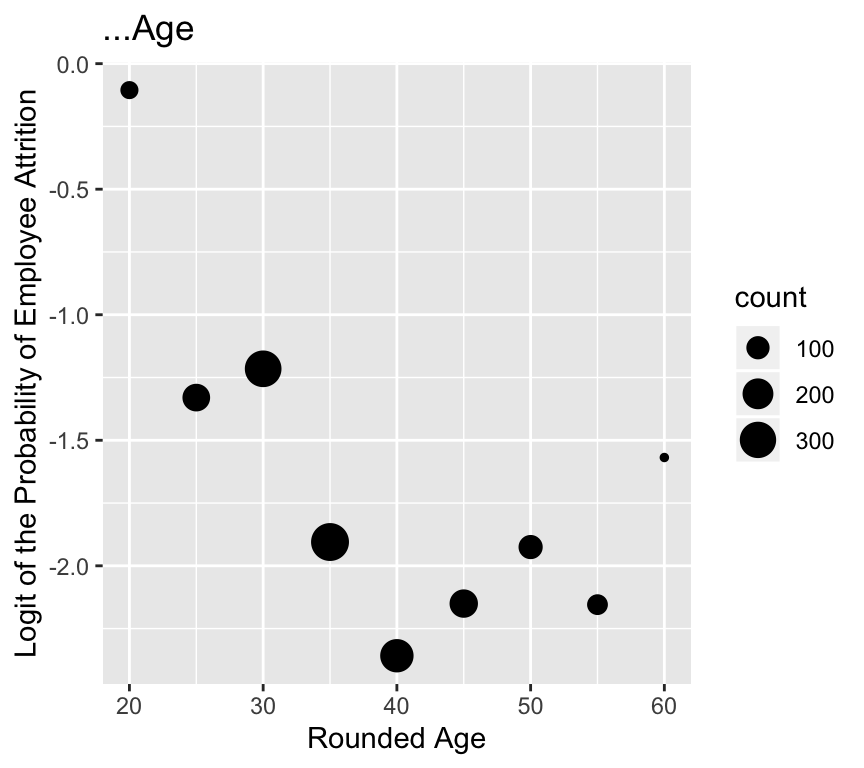
\includegraphics{EmployeeAttrition_files/figure-latex/unnamed-chunk-3-1.pdf}
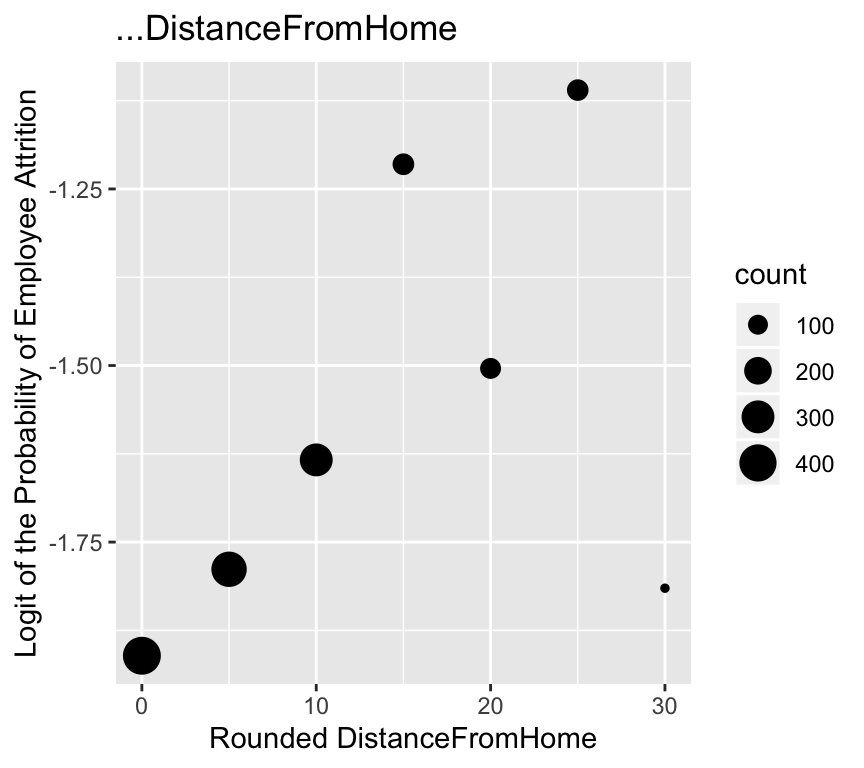
\includegraphics{EmployeeAttrition_files/figure-latex/unnamed-chunk-3-2.pdf}
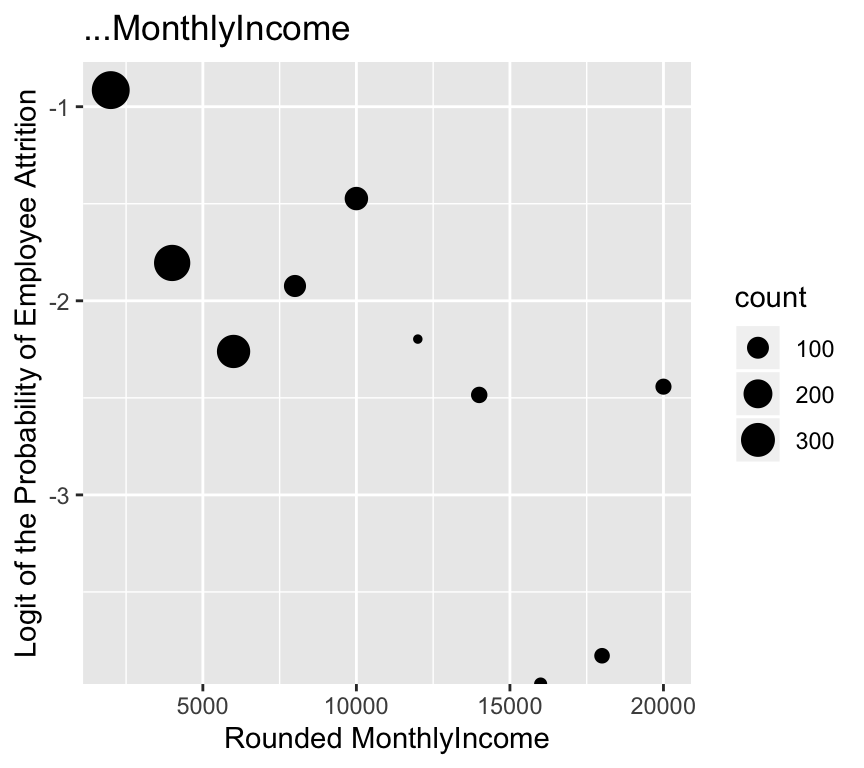
\includegraphics{EmployeeAttrition_files/figure-latex/unnamed-chunk-3-3.pdf}
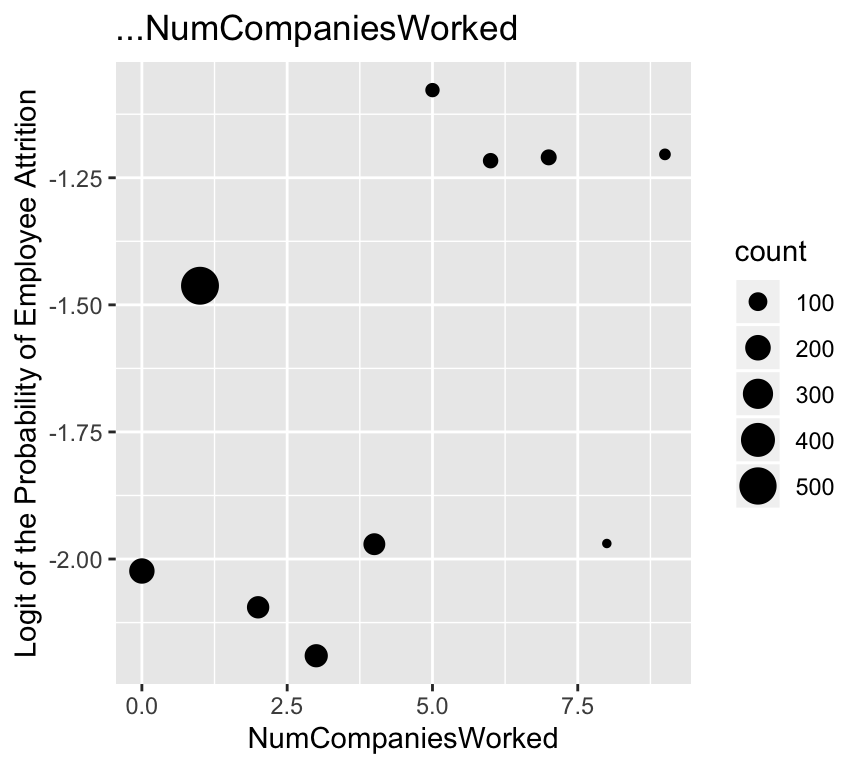
\includegraphics{EmployeeAttrition_files/figure-latex/unnamed-chunk-3-4.pdf}
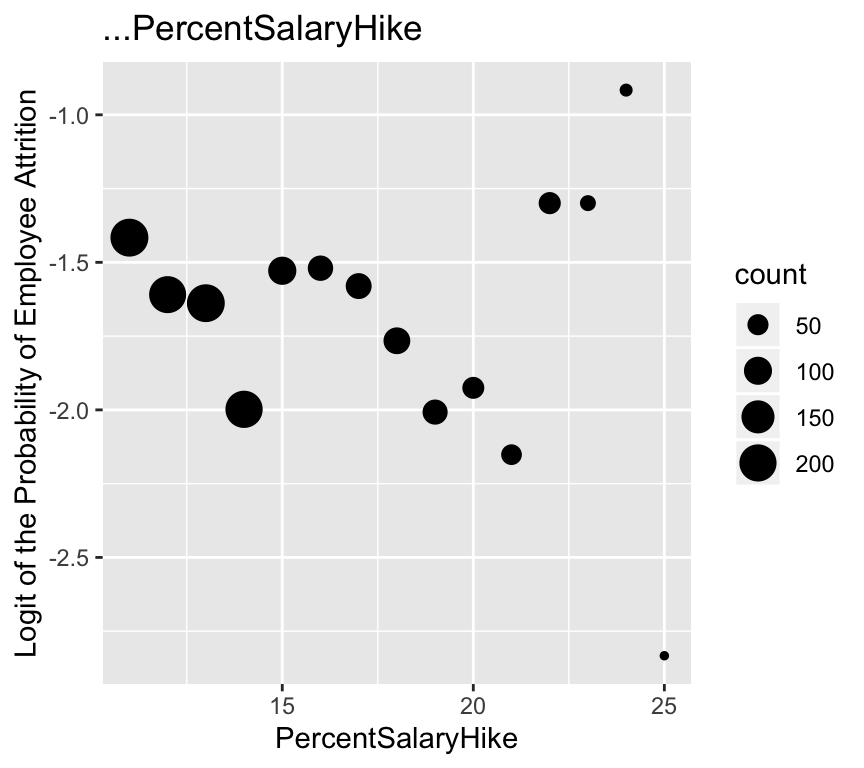
\includegraphics{EmployeeAttrition_files/figure-latex/unnamed-chunk-3-5.pdf}
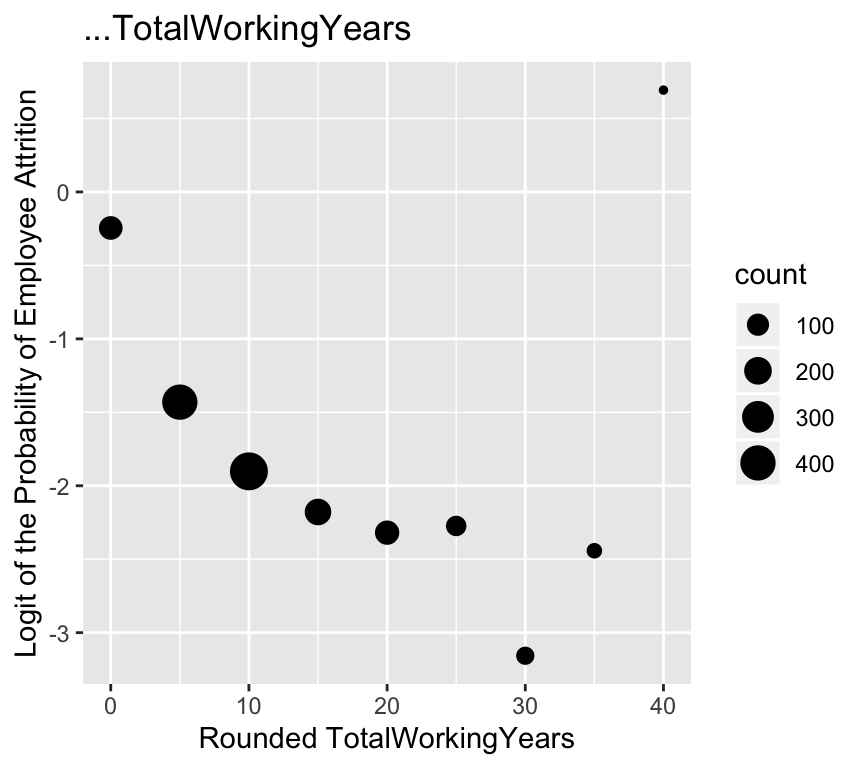
\includegraphics{EmployeeAttrition_files/figure-latex/unnamed-chunk-3-6.pdf}
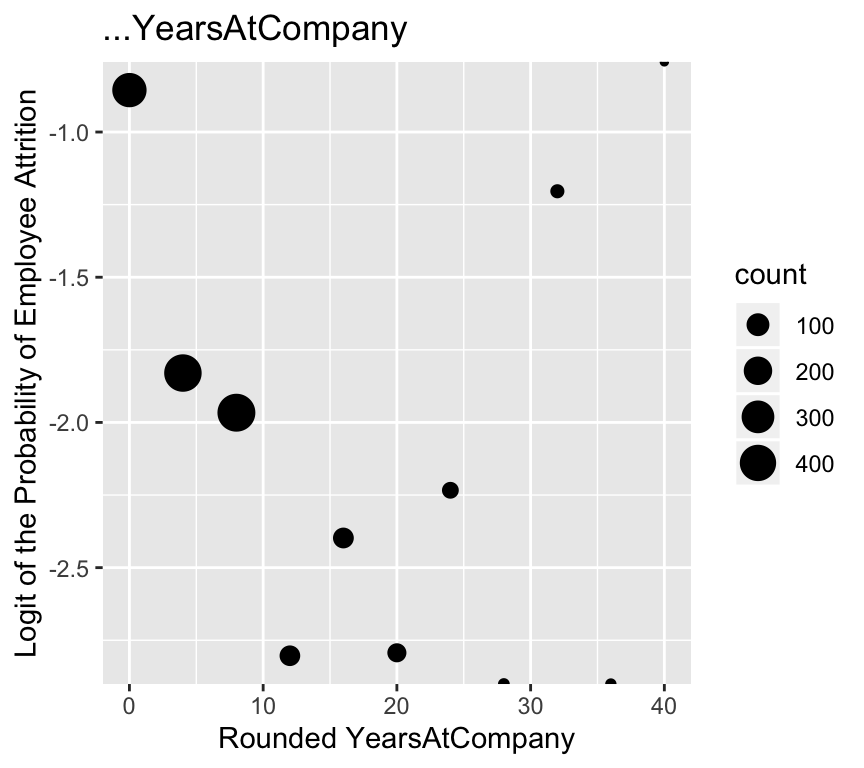
\includegraphics{EmployeeAttrition_files/figure-latex/unnamed-chunk-3-7.pdf}
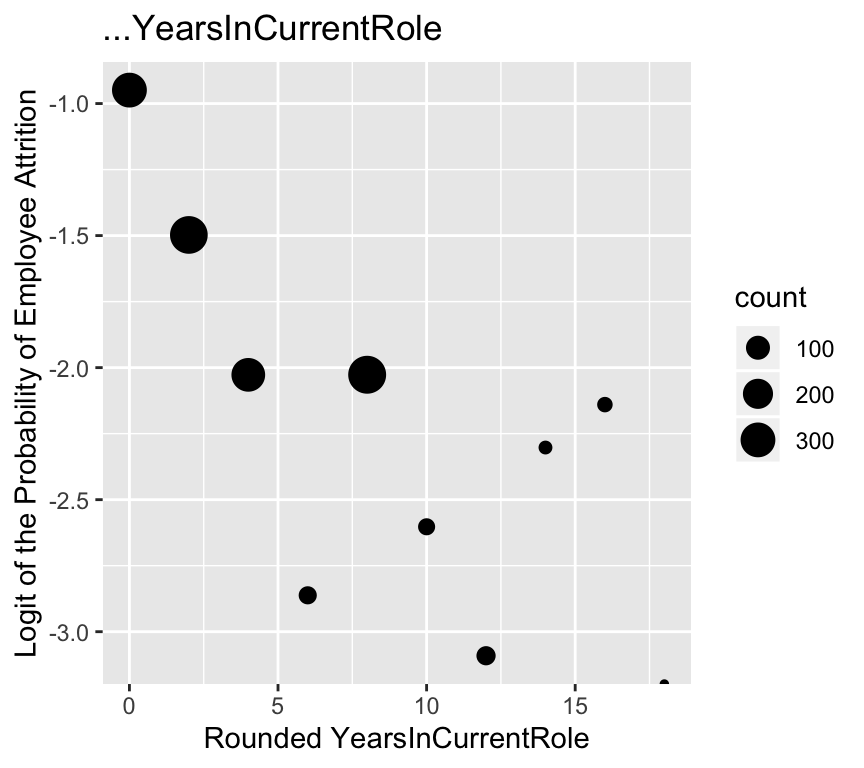
\includegraphics{EmployeeAttrition_files/figure-latex/unnamed-chunk-3-8.pdf}
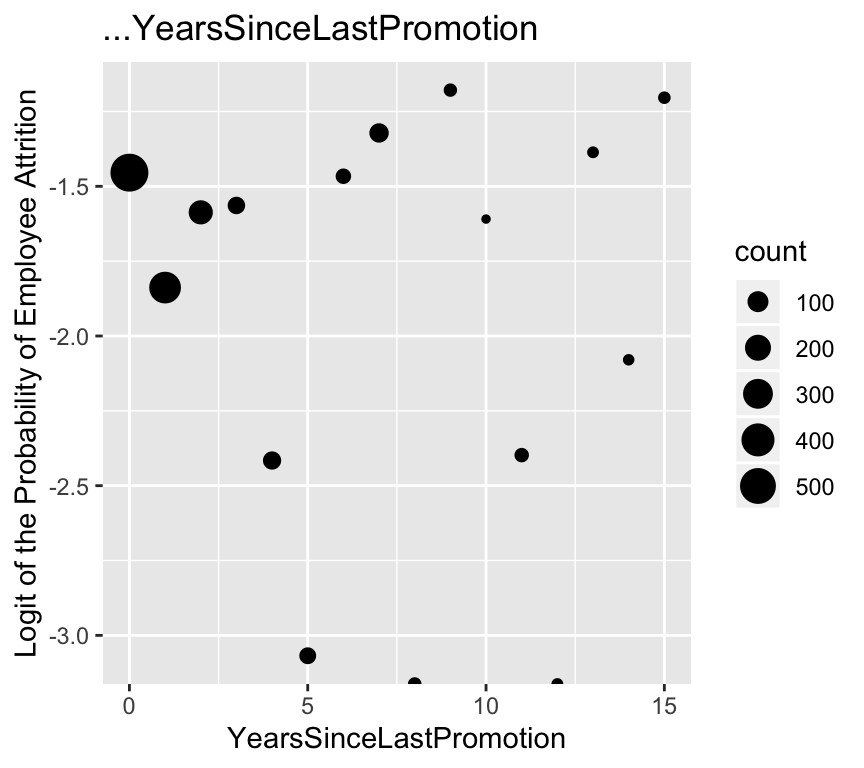
\includegraphics{EmployeeAttrition_files/figure-latex/unnamed-chunk-3-9.pdf}
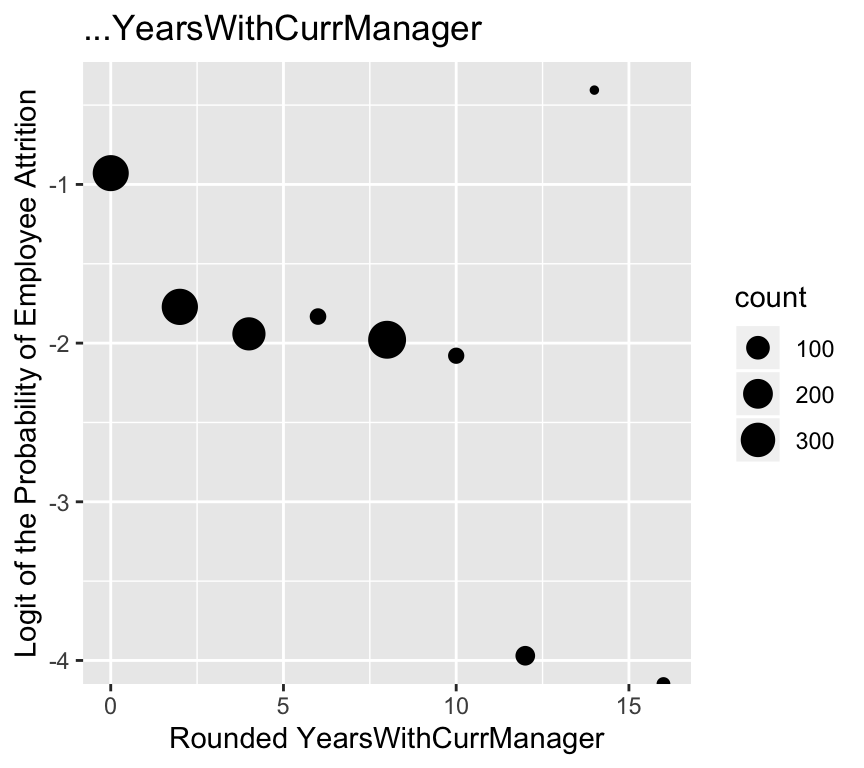
\includegraphics{EmployeeAttrition_files/figure-latex/unnamed-chunk-3-10.pdf}

It may be worth looking at the relationship between the logit of the
probability and an inverse transformation of TotalWorkingYears due to
the exponential trend. However, TotalWorkingYears includes values of `0'
and the inverse of these are NaN. The current trend is not too
exponential and is still reasonably linear enough to suggest a
relaionship.

We can see from these plots that several of the covariates appear to
have a linear relationship with the logit of the probability of employee
attrition. In particular, age, distance from home, monthly income, total
working years, and years in current role look to be associated with the
logit. Additionally, the points in these plots that follow the linear
trend are typically larger in size and the size is based on the size of
the group. This suggests that the other smaller points that deviate from
the linear trend may be doing so as a result of their small grouping
size, as opposed to failing to follow the same pattern.

Beyond this, it is worth exploring possible interactions between terms
that may be taking place:

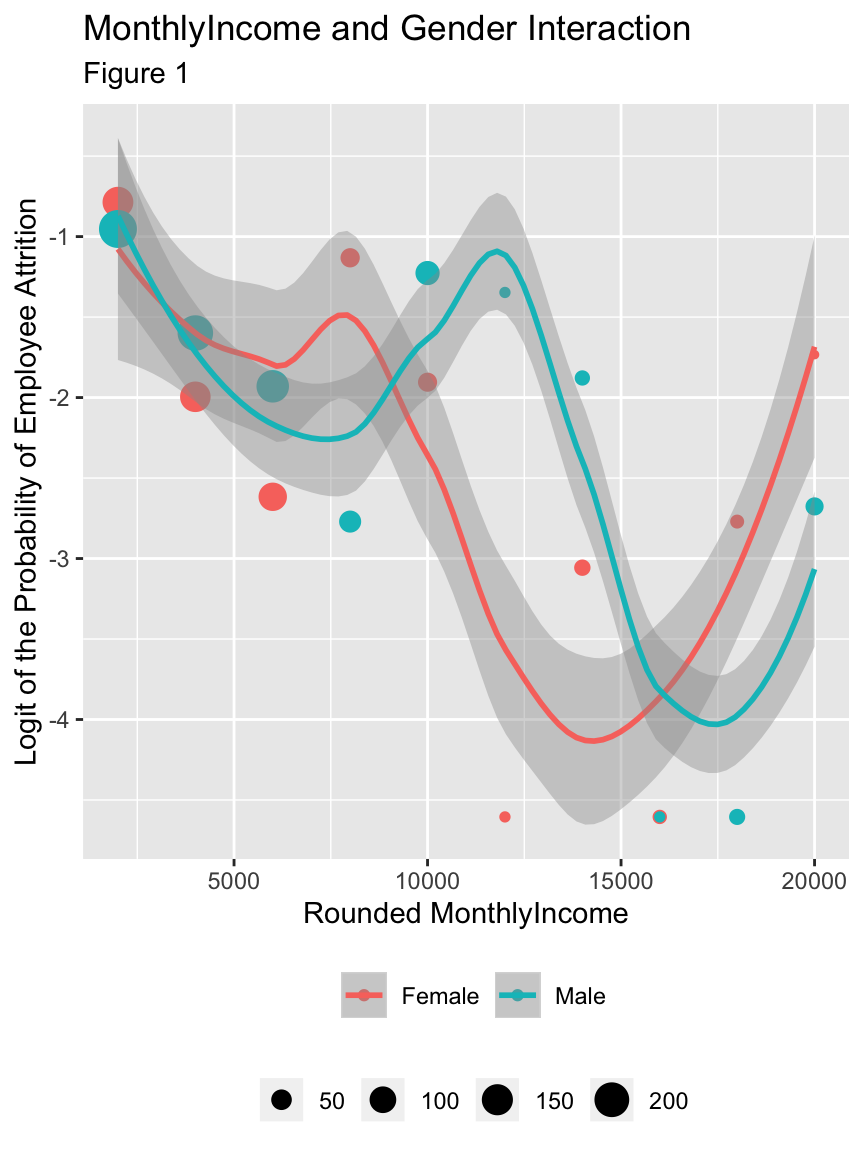
\includegraphics{EmployeeAttrition_files/figure-latex/unnamed-chunk-4-1.pdf}
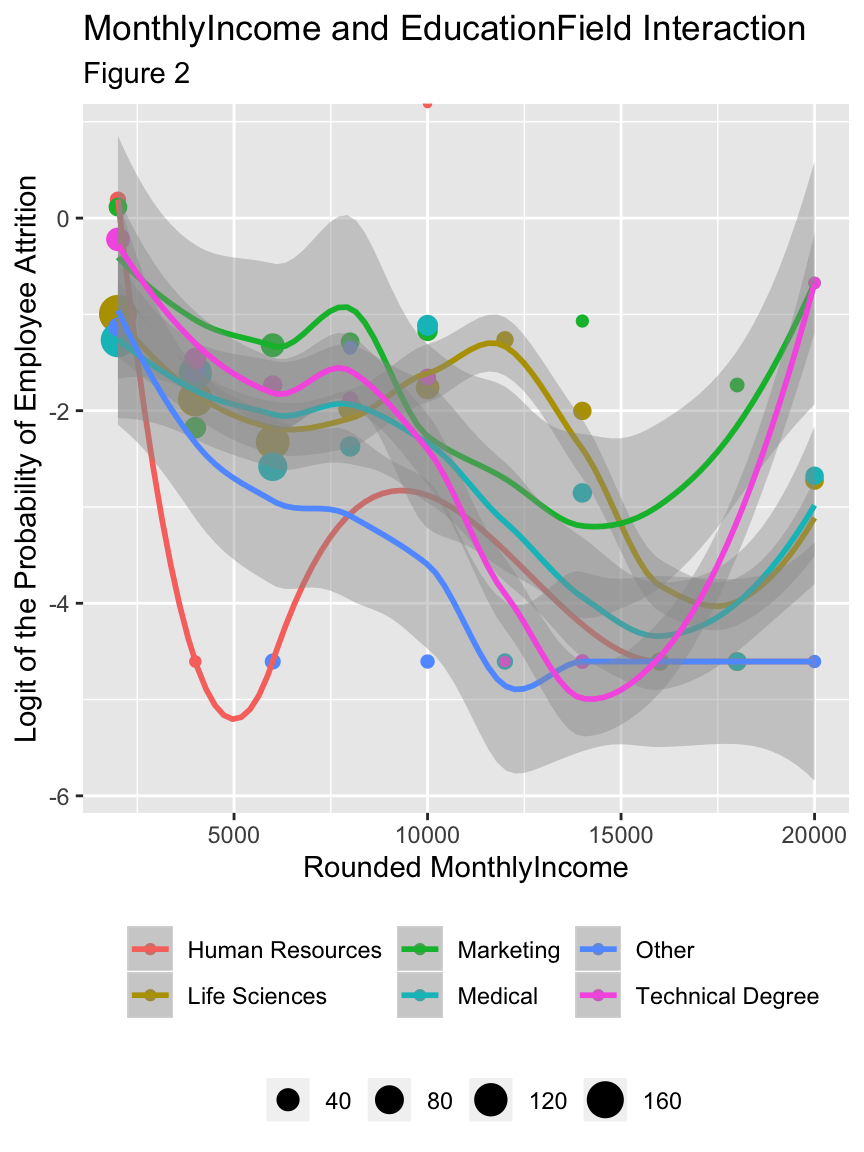
\includegraphics{EmployeeAttrition_files/figure-latex/unnamed-chunk-4-2.pdf}
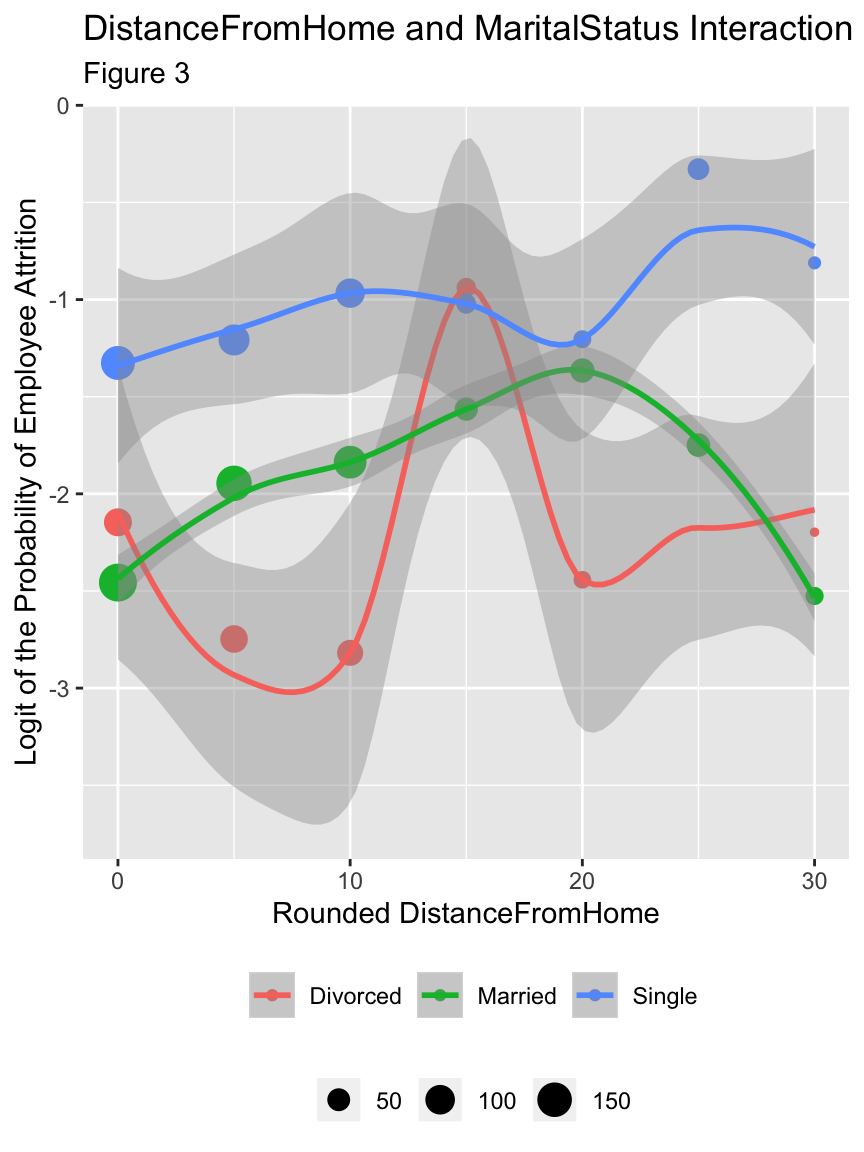
\includegraphics{EmployeeAttrition_files/figure-latex/unnamed-chunk-4-3.pdf}
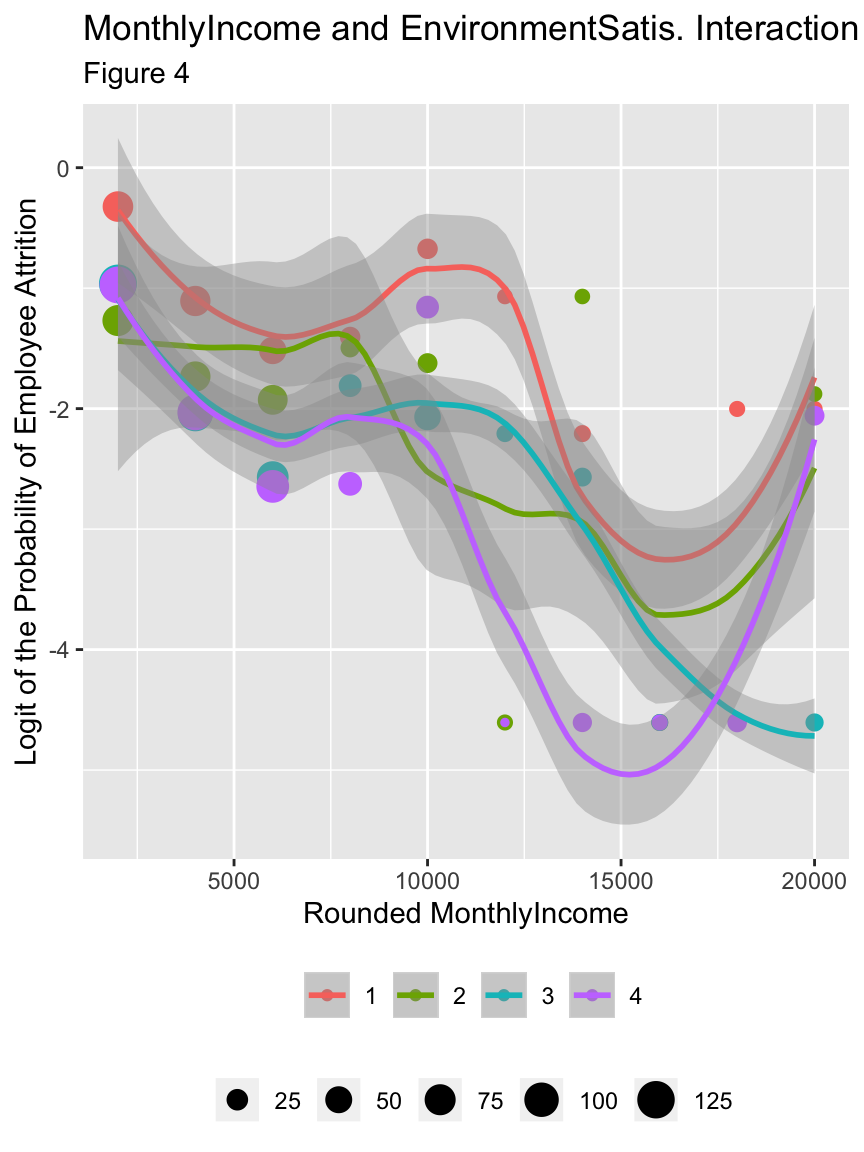
\includegraphics{EmployeeAttrition_files/figure-latex/unnamed-chunk-4-4.pdf}
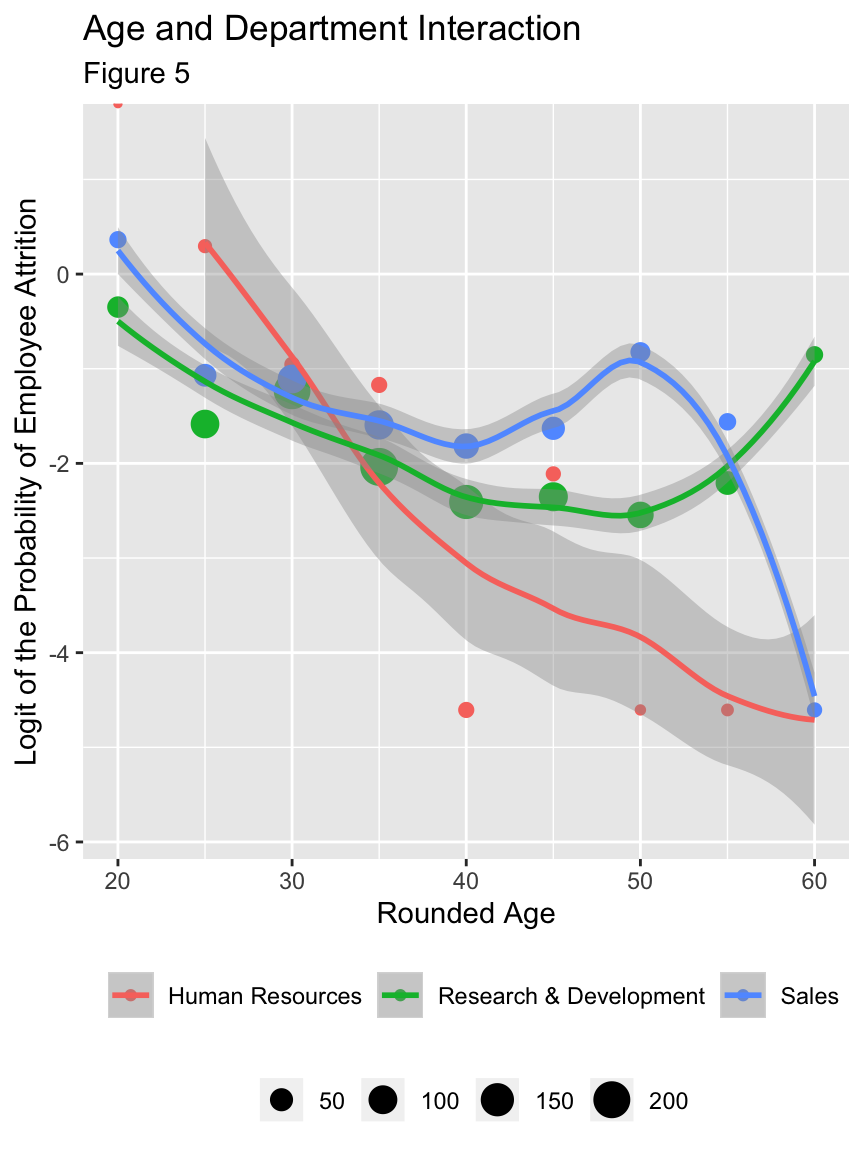
\includegraphics{EmployeeAttrition_files/figure-latex/unnamed-chunk-4-5.pdf}
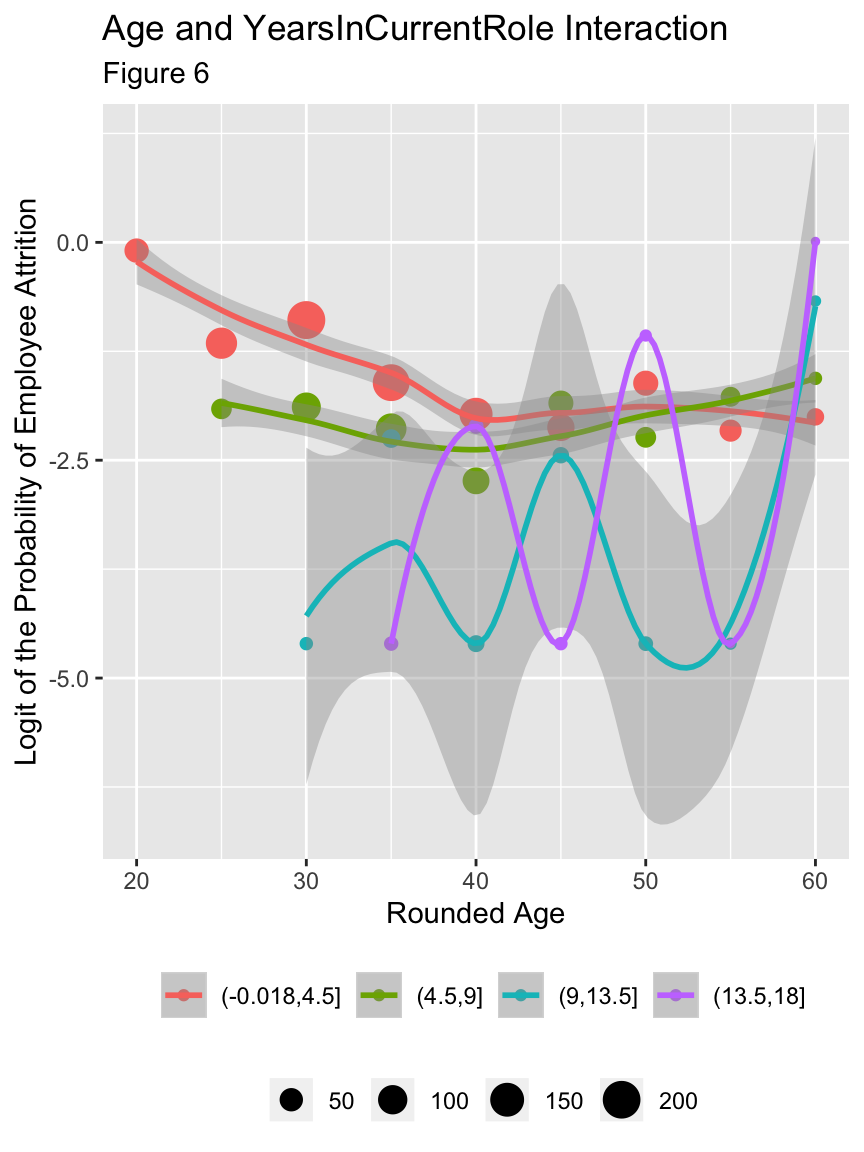
\includegraphics{EmployeeAttrition_files/figure-latex/unnamed-chunk-4-6.pdf}

These interaction plots are able to provide us with some more insight
into how the covariates may be interacting with each other, or not, in
determining the logit of the probability of employee attrition. All of
these plots include confidence interval shading at the 50\% confidence
level.

There does not appear to be much of an interaction in figure 1 between
the monthly income of an employee and their gender for the logit of the
probability. There may be some linear trends present for each individual
gender but the slope of those look to be similar for any linear trend.

When looking at the plot in figure 2 with an employee's monthly income
and their education there doesn't seem to be any linear associations
present. There looks to be a potential cubic trend for the life sciences
field, but overall monthly income doesn't appear to interact with
education field for the logit.

In figure 3, an employee's marital status does appear to be correlated
with their distance from home and possess a linear relationship with the
logit. However, the slopes for those who are single or married appear to
be similar or the some. There isn't a strong linear relationship for
those who have been divorced but the presence of linear relationships
across factor values is still promising.

There does appear to be some differing correlations between the logit
and monthly income based on am employee's environment satisfaction (with
1 being the lowest and 4 being the highest) in figure 4. In order words,
there is reason to believe there may be different slopes for each
different satisfaction level's relationship between monthly income and
logit of the probability of attrition. However, the points are still
scattered and scarce enough to prevent certainty.

Another interaction looked at was between the age and department of an
employee in figure 5. The interaction plot shows linear relationships
between the logit and age for each department. However, the slope of the
trend for each department looks to be similar. Therefore, there may not
be much of an interaction going on between age and department, but age
still looks to be associated with the logit.

Lastly in figure 6, there looks to be some linear trends going on across
age for each color, or cut of 4.5 years for years that an employee has
been in their current role. Furthermore, the slopes for these linear
trends across age appear to be different for each year group. The number
of points for the two longest tenured group is small so we can't be
completely confident, but the current look may suggest an interaction
between age and years in current role.

\hypertarget{model-building}{%
\section{Model Building}\label{model-building}}

Based on our insight from the marginal and joint interaction plots
against the logit we begin with an initial model and build off of it
using model summaries and ANOVA tables to determine the useful and less
impactful variables and interactions in the model. We will use model
building to better understand what seems to lead to employee attrition.

\hypertarget{initial-model}{%
\subsubsection{Initial Model}\label{initial-model}}

Our initial model will include each continuous main effect that looked
to be correlated in the marginal logit plots (age, distance from home,
monthly income, years in current role, and total working years).
Additionally, we will include an interaction between distance from home
and marital status. This interaction showed linear relationships but
potentially similar slopes in its plot, so it is worth exploring more.

The only significant covariates in this model are the marital status of
single factor variable, age, monthly income, and years in current role
(all at \(\alpha = 0.05\) level) and the intercept at the
\(\alpha = 0.01\) level. Also, the AIC of this model is 1199.4. The
analysis of deviance tells us that the sequential addition of each
variable is useful in the model except for total working years and the
interaction term. Since the individual terms in the interaction are
significant we will only drop their interaction, along with the total
working years term.

\hypertarget{remove-totalworkingyears-add-businesstravel-remove-interaction}{%
\subsubsection{Remove TotalWorkingYears, add BusinessTravel, remove
interaction}\label{remove-totalworkingyears-add-businesstravel-remove-interaction}}

Since we have assessed many of the continuous variables with the logit
plots it will be helpful to consider the impact of the factor variables
in the data when model building. Therefore, our next model includes the
business travel factor variable in place of the total working years
variable and no interaction between distance from home and marital
status.

Every term in this model is significant at the \(\alpha = 0.05\) level
except for the marital status of married factor variable (which has no
significance). The AIC of this model is an improvement at 1173.5.
Additionally, our analysis of deviance tells us that the addition of
each variable in the model is significant. With the impact of each
individual factor level in mind we will alter the marital status
variable into an isSingle variable that indicates `1' for cases when an
employee is single and `0' otherwise.

\hypertarget{switch-out-maritalstatus-for-issingle}{%
\subsubsection{Switch out MaritalStatus for
isSingle}\label{switch-out-maritalstatus-for-issingle}}

This model is the same as the previous except for the replacement of the
MaritalStatus term with the isSingle variable.

Every term in this model is still significant, including the new
isSingle factor variable that remains as significant as the `single'
factor level did in the marital status variable. The AIC of this model
is a slight improvement at 1172.7. The switching of the factor term was
not exactly necessary then but it may help to simplify the model
overall. The analysis of deviance continues to signify that the addition
of each variable in the model is worthy.

\hypertarget{add-department}{%
\subsubsection{Add Department}\label{add-department}}

Although the department of an employee didn't appear to interact with
age, the department factor still appears to be associated with the logit
of the probability when it is looked at through an employees age.
Therefore, we will add the department factor variable into the model.

After adding this variable the AIC drops from 1172 to 1162. However, the
only variables that aren't significant in the model are the two
department factor variable that aren't the baseline. The analysis of
deviance shows that the addition of the department variable after all
others is still significant in the model. The AIC suggests this model is
a better mix of model fit and model complexity but with so many
covariate options we would prefer to only choose those that are
significant for explaining the logit of the probability of attrition.
Another variable to consider is how many companies an employee has
worked for. The marginal plot for this variable did not possess a linear
relationship with the logit, but there does look to be two separate
chunks in the plot. These chunks tell the story that those who have
worked at more companies are more likely to leave the current company
and, again, work for another company. The other chunk represents those
who have worked for less companies and are correspondingly less likely
to leave the company.

\hypertarget{remove-department-add-numcompaniesworked}{%
\subsubsection{Remove Department, add
NumCompaniesWorked}\label{remove-department-add-numcompaniesworked}}

This model possess all other covariates as before excpet the department
term and includes the number of companies an employee has worked for
instead.

The AIC for this model with number of companies worked for instead of
department is also at 1162. This time all of the variables are
significant in the model, and the deviance analysis confirms that the
inclusion of each variable (including NumCompaniesWorked after
everything else) is significant in the model.

\hypertarget{add-yearssincelastpromotion}{%
\subsubsection{Add
YearsSinceLastPromotion}\label{add-yearssincelastpromotion}}

Another variable that makes sense to try in the model that could lead to
an employee leaving a company in how long it has been since the employee
has been promoted. There are several variables with the same theme as
this one in YearsAtCompany, YearsInCurrentRole, and
YearsWithCurrManager. The marginal plot of years since promotion and the
logit doesn't suggest a strong linear relationship but it is still worth
checking if we can explain more of the variability.

The AIC for this model with the addition of YearsSinceLastPromotion
variable is 1146.3. This is lower then the model we previously had which
is good. All of the variables in this model seem to be significant and
the deviance analysis confirms that the addition of
YearsSinceLastPromotion seems to be significant in the model. The next
variable we would want to look at is JobSatisfaction and see if that
variable is significant or not in attrition.

\hypertarget{add-jobsatisfaction-as-a-factor-variable}{%
\subsubsection{Add JobSatisfaction as a factor
variable}\label{add-jobsatisfaction-as-a-factor-variable}}

Another factor variable that is worth checking on in the model that was
not looked at in the EDA is how satisfied an employee is with their job.
It makes sense that an employee who is less satisfied with their job is
more likely to leave the company, and vice versa.

When we make JobSatisfaction a factor variable, the AIC in this model
becomes 1130.9. Again, the AIC is decreasing which is showing signs of
improvement in our model building. All of the variables in the model
seem to be significant and the deviance analysis confirms this as well.
This model analysis tells us that making JobSatisfaction a factor
variable is significant and necessary. To help make understand and
interpreting this model easier, we want to see if looking at a specific
JobSatisfaction rating has an impact on attrition.

\hypertarget{replace-jobsatisfaction-variable-with-issatisfied}{%
\subsubsection{Replace JobSatisfaction variable with
isSatisfied}\label{replace-jobsatisfaction-variable-with-issatisfied}}

Since job satisfaction ratings of 2 and 3 (on a scale from 1 to 4) were
significant at the \(\alpha = 0.05\) level and a satisfaction rating of
4 was significant at the \(\alpha = 0.001\) level we created an
isSatisfied term to signal if an employee was either fully satisfied
with a rating of 4, or not.

In this model, we replaced JobSatisfaction with isSatisfied. With this
switch, our AIC became 1133.6 which is a little higher compared to the
AIC in the previous model. Even though the AIC is a bit higher, the
deviance analysis confirms that all the variables are significant and
neccesary in the model and the model arguably becomes more simple with
less overall main effect terms. Even though this is a good model, there
are no intereaction terms so the next model would have Age and
YearsInCurrentRole as interaction variables to see if there is an
interaction between the two and if there is a significance.

\hypertarget{include-interaction-between-age-and-yearsincurrentrole}{%
\subsubsection{Include interaction between Age and
YearsInCurrentRole}\label{include-interaction-between-age-and-yearsincurrentrole}}

Out of the interactions that we looked at in EDA one of the plots that
showed potential for an interaction was between age and the number of
years an employee has been in their current role. These are two
significant variables that we already have in our model, therefore we
will add an interaction between them to assess the impact.

In the final model that we created, we included an interaction between
Age and YearsInCurrentRole. With this interaction term added, the AIC
dropped down to 1119.5. This is the lowest AIC thus far when comaparing
to all the other models that were created. All of the variables in this
model are highly significant. The analysis of the deviance table support
the addition of the interaction term between Age and YearsInCurrentRole,
as it is still seen as useful after the addition and variability
explained by the prior covariates.

\hypertarget{add-worklifebalance-factor-variable}{%
\subsubsection{Add WorkLifeBalance factor
variable}\label{add-worklifebalance-factor-variable}}

Lastly, we consider another factor variable to add into the model. This
variable measures on a scale from 1 to 4 what an employee's work-life
balance is. This term is reasonable to consider because those with a
less healthy work-life balance may be more inclined to change who they
work for. Similarly, those who note a more healthy work-life balance may
be less likely to leave a company.

Every variable in this model is significant at least at the
\(\alpha = 0.05\) level, while most are significant at the
\(\alpha = 0.001\) level. Additionally, the analysis of deviance again
confirms that the addition of this factor term is useful in the model.
The AIC for this model makes another drop to 1110.8. We now have 10
variables in our model and have continued to move are AIC down while
maintaining significant variables. We will move forward with this model
for diagnostics.

\hypertarget{model-selection}{%
\section{Model Selection}\label{model-selection}}

We choose to move forward with the last model including the
DistanceFromHome continuous, isSingle factor, Age continuous and
YearsInCurrentRole continuous interaction, MonthlyIncome continuous,
BusinessTravel factor, NumCompaniesWorked continuous,
YearsSinceLastPromotion continuous, isSatisfied factor, and
WorkLifeBalance factor variables. The AIC for this final model is
1110.8. Each term in the model is significant at the \(\alpha = 0.05\)
level, and the analysis of deviance confirms that the sequential
inclusion of each covariate in the model is significant (at the
\(\alpha = 0.01\) level). The following table shows what the
significance of each covariate in the model is after accounting for the
variables that come before it. This deviance analysis for each model
helps to understand which terms contribute to the unexplained
variability in what leads to an employee leaving a company.

\begin{tabular}{l|r}
\hline
Variable & Significance\\
\hline
DistanceFromHome & 0.010\\
\hline
isSingle & 0.001\\
\hline
Age & 0.001\\
\hline
YearsInCurrentRole & 0.001\\
\hline
MonthlyIncome & 0.010\\
\hline
BusinessTravel & 0.001\\
\hline
NumCompaniesWorked & 0.001\\
\hline
YearsSinceLastPromotion & 0.001\\
\hline
isSatisfied & 0.001\\
\hline
WorkLifeBalance & 0.010\\
\hline
Age:YearsInCurrentRole & 0.001\\
\hline
\end{tabular}

\hypertarget{diagnostics}{%
\section{Diagnostics}\label{diagnostics}}

We will now plot the residuals of our model against several variables in
the data that are not included in the model. This is done in order to
see if a variable has a (higher order) relationship with the deviance
residuals and should be included in the model:

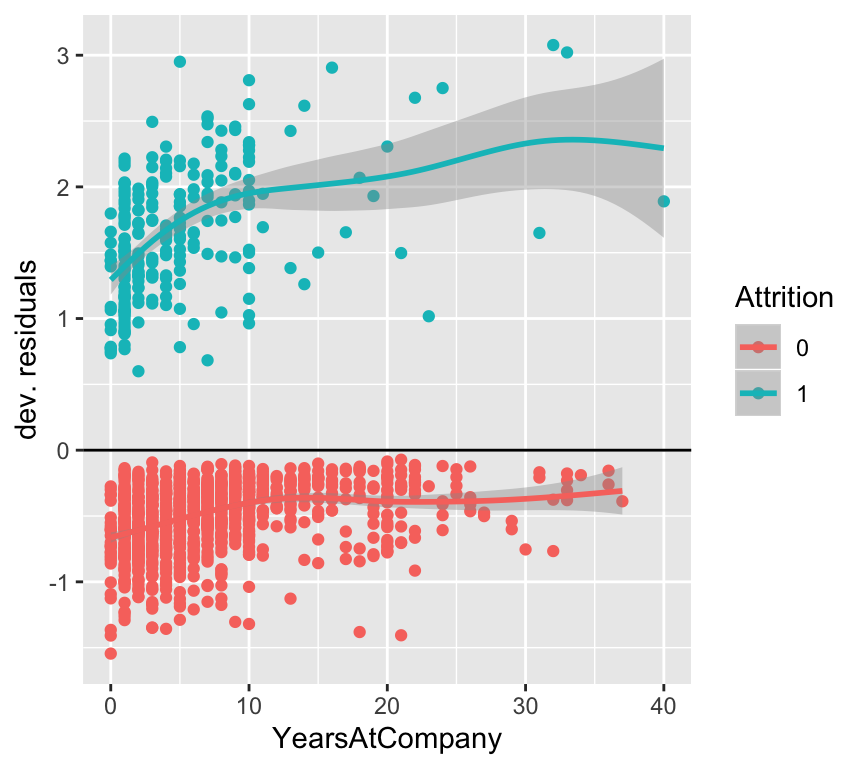
\includegraphics{EmployeeAttrition_files/figure-latex/unnamed-chunk-27-1.pdf}
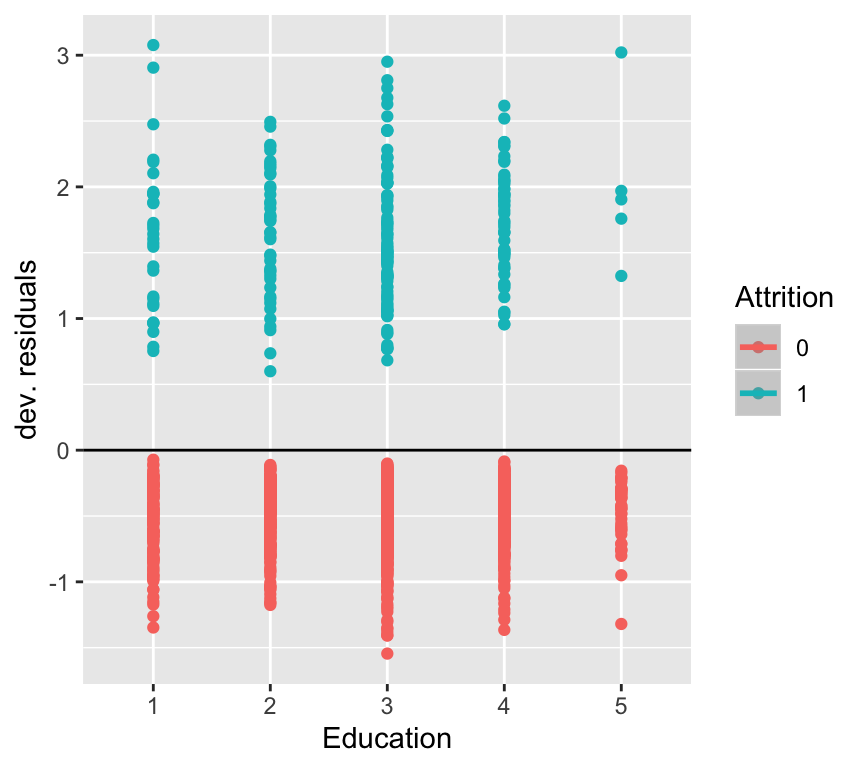
\includegraphics{EmployeeAttrition_files/figure-latex/unnamed-chunk-27-2.pdf}

There looks to be a potential linear trend between the number of years
an employee has been at the company and the residuals (for those who did
end up leaving). This trend could suggest that YearsAtCompany may be
useful in the model and is worth looking into. The plot for education
versus the residuals is like many of the other plots left out of the
report. The variance of the residuals over each factor level looks to be
consistent and does not suggest the respective variable (Education in
this case) is necessary in the model.

\begin{center}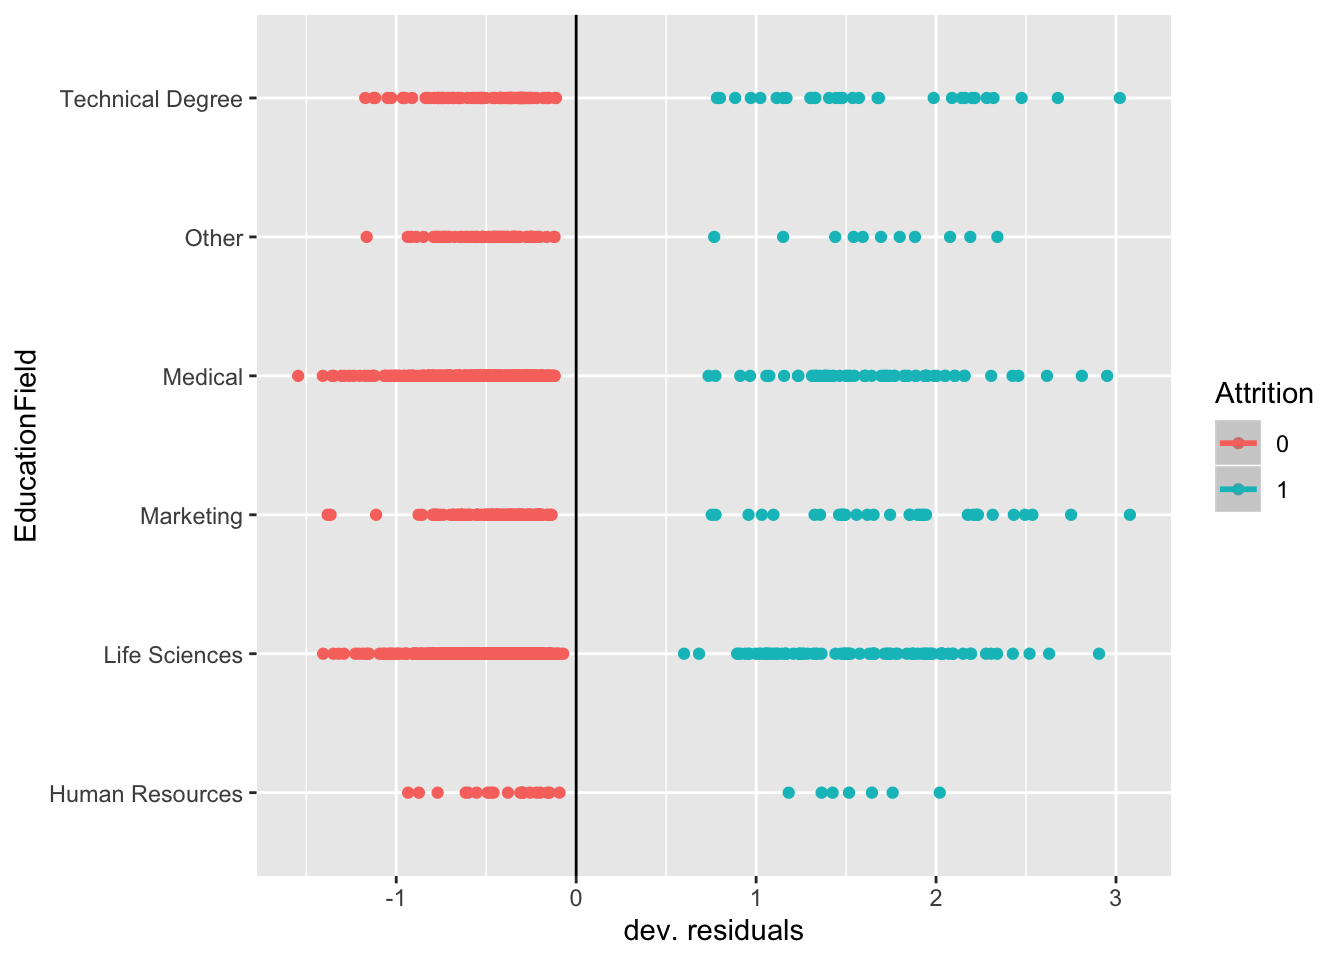
\includegraphics{EmployeeAttrition_files/figure-latex/unnamed-chunk-28-1} \end{center}

The deviance residuals don't appear to vary much over the different
education fields and so this variable is likely not very useful in the
model.

\begin{center}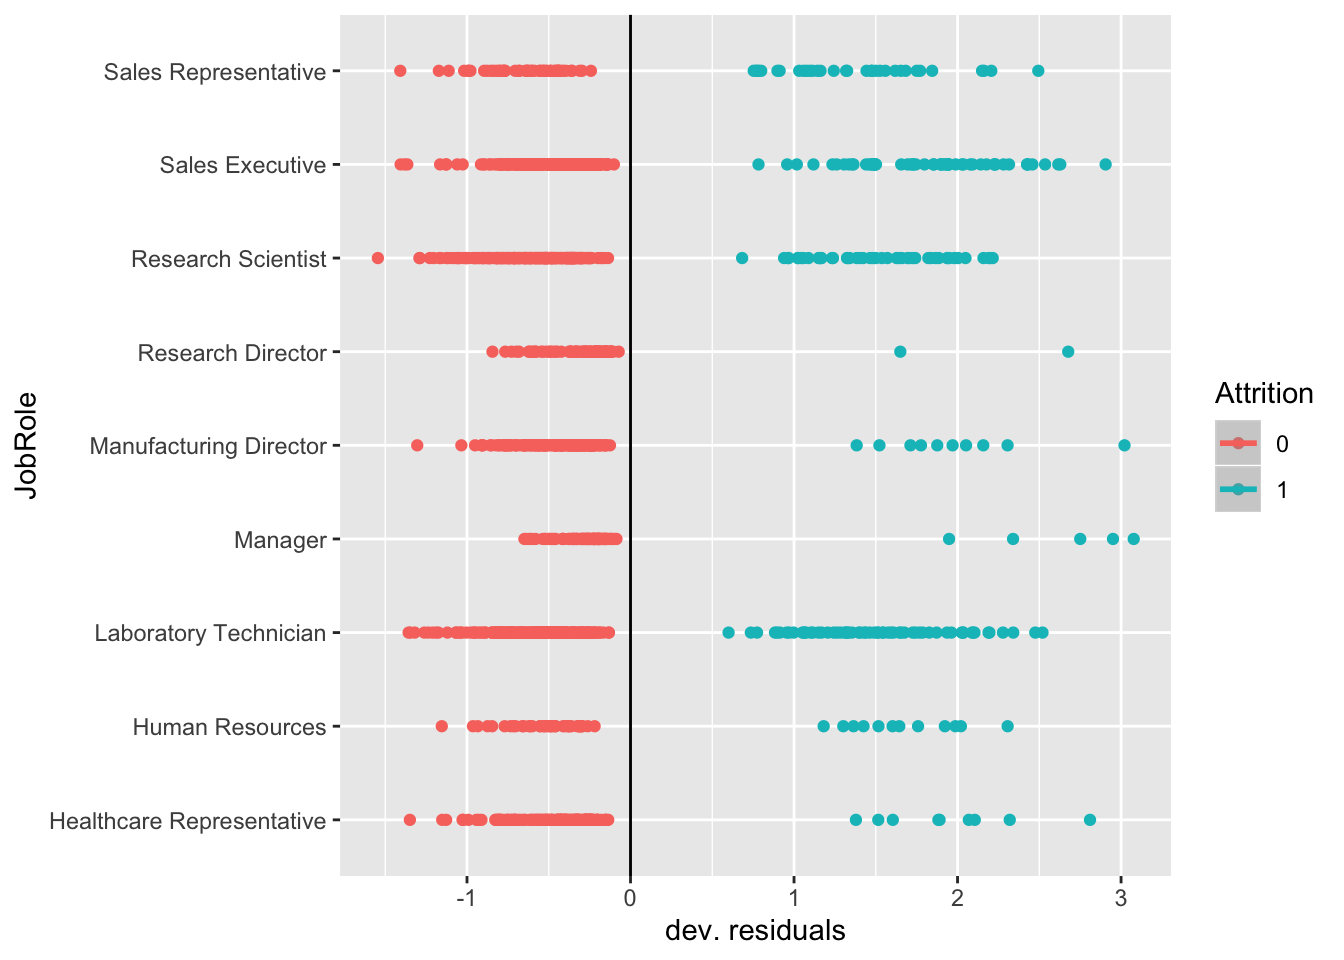
\includegraphics{EmployeeAttrition_files/figure-latex/unnamed-chunk-29-1} \end{center}

Similarly, the residuals appear to vary consistently over the different
job roles. The only noticeable pattern is that those in higher level
positions (managers/directors) do not appear to leave the company as
often as other roles. The inclusion of a factor variable that separates
managers and directors from other roles may be useful in determining
employee attrition but we are content with our current model.

We will now add YearsAtCompany into our chosen model in order to assess
its impact.

The AIC for this model with all of the prior terms and YearsAtCompany
increases from 1110 to 1112. Furthermore, the model summary shows that
the only variable that is not significant in the model is this newly
added term. The deviance analysis also shows that this YearsAtCompany
variable is the only variable not worth adding into the model after
considering the impact of prior covariates. Therefore, we will remove
this term and keep our other model that seems to explain decent
variability.

\hypertarget{results}{%
\section{Results}\label{results}}

An increase in age of one year is associated with a multiplicative
change of \(e^{-.07132 + .01039 \times YearsInCurrentRole}\) in employee
attrition for a given YearsInCurrentRole.

\end{document}
